% image-kinds — one image of each kind a document holds, each under its caption's text.
%
% One concern, issue #11's: an image becomes the Markdown that carries what it holds. The four
% kinds, in the order the page sets them:
%
%   - text: image-kinds-text.png, a paragraph set as type and rasterised. Its words are the gold.
%   - a table: image-kinds-table.png, a ruled table rasterised. Its grid is the gold.
%   - a chart: image-kinds-chart.png, a bar chart of four labelled values. The table of those
%     values is the gold, since that is what the chart says; reading it takes a model.
%   - a picture: image-bands.png, image.tex's three flat colour bands. No text is the answer,
%     so the gold marks it [image]; a description is a model's and is not gold.
%
% Every image is PNG under /FlateDecode at 200 dpi, so nothing on the page but the prose and
% the captions is text in the content stream. The images are built from the image-kinds-*.tex
% sources; see README.md.
\documentclass{article}
\usepackage{lmodern}
\usepackage{graphicx}
\pagestyle{empty}
\setlength{\parindent}{0pt}
\setlength{\parskip}{8pt}
\begin{document}

Each kind of image a document holds, one after another.

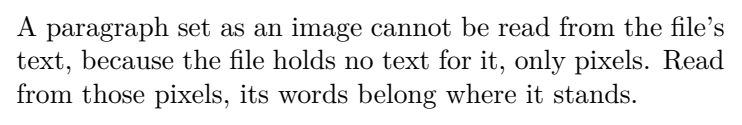
\includegraphics[width=9cm]{image-kinds-text.png}

Figure 1: text set as an image.

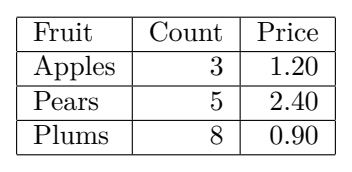
\includegraphics[width=8cm]{image-kinds-table.png}

Figure 2: a table set as an image.

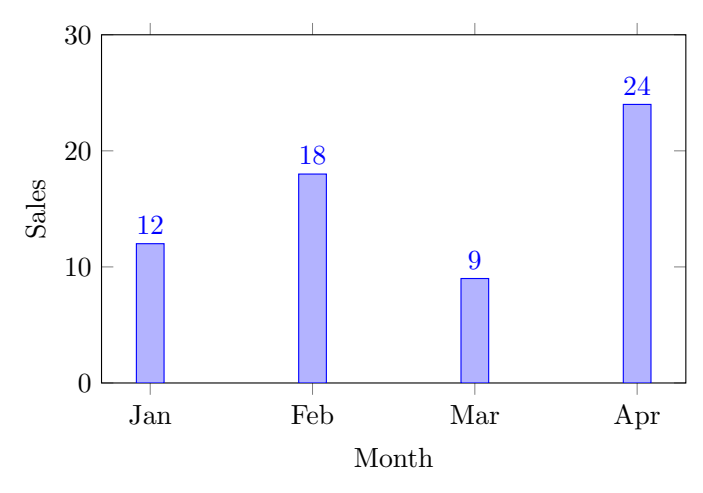
\includegraphics[width=8cm]{image-kinds-chart.png}

Figure 3: a bar chart.


\includegraphics[width=4cm]{image-bands.png}

Figure 4: three colour bands.

\end{document}
